\documentclass[border=8pt]{standalone}
\usepackage{tikz}
\usetikzlibrary{arrows.meta,positioning,calc,fit}
\begin{document}
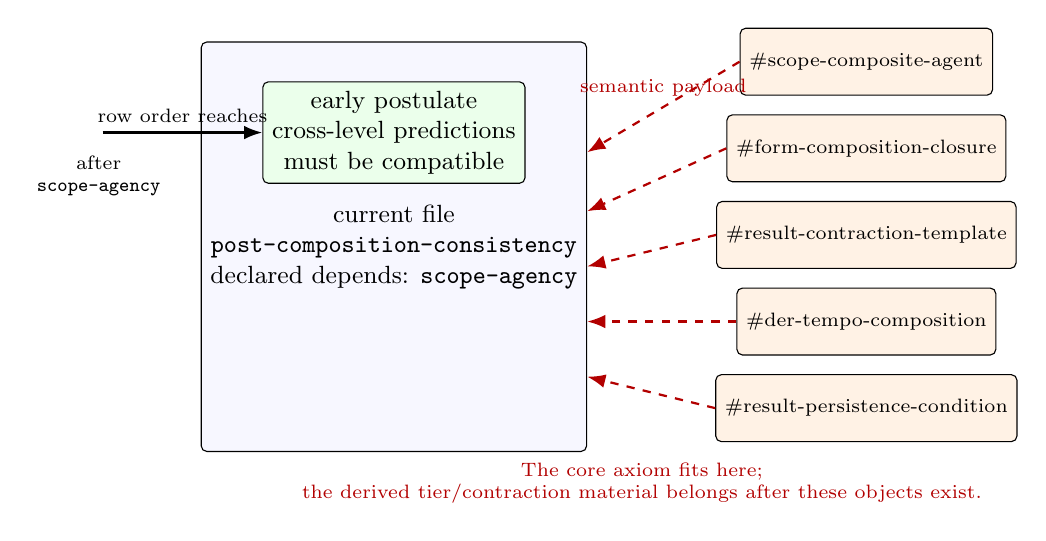
\begin{tikzpicture}[
  core/.style={draw, rounded corners=2pt, align=center, minimum width=3.1cm, minimum height=1.1cm, font=\small, fill=green!8},
  future/.style={draw, rounded corners=2pt, align=center, minimum width=2.7cm, minimum height=0.85cm, font=\scriptsize, fill=orange!10},
  file/.style={draw, rounded corners=2pt, align=center, minimum width=4.0cm, minimum height=5.2cm, font=\small, fill=blue!3},
  arr/.style={-Latex, thick},
  dep/.style={-Latex, thick, dashed, red!70!black},
  note/.style={align=center, font=\scriptsize}
]

\node[file] (seg) at (0,0) {current file\\\texttt{post-composition-consistency}\\declared depends: \texttt{scope-agency}};
\node[core] (core) at (0,1.45) {early postulate\\cross-level predictions\\must be compatible};

\node[future] (scope) at (6,2.35) {\#scope-composite-agent};
\node[future] (closure) at (6,1.25) {\#form-composition-closure};
\node[future] (template) at (6,0.15) {\#result-contraction-template};
\node[future] (tempo) at (6,-0.95) {\#der-tempo-composition};
\node[future] (persist) at (6,-2.05) {\#result-persistence-condition};

\draw[dep] (scope.west) -- node[above, note] {semantic payload} ($(seg.east)+(0,1.2)$);
\draw[dep] (closure.west) -- ($(seg.east)+(0,0.45)$);
\draw[dep] (template.west) -- ($(seg.east)+(0,-0.25)$);
\draw[dep] (tempo.west) -- ($(seg.east)+(0,-0.95)$);
\draw[dep] (persist.west) -- ($(seg.east)+(0,-1.65)$);

\node[note, red!70!black] at (3.15,-3.0) {The core axiom fits here;\\the derived tier/contraction material belongs after these objects exist.};

\draw[arr] (-3.7,1.45) -- node[above, note] {row order reaches} (core.west);
\node[note] at (-3.75,0.9) {after\\\texttt{scope-agency}};

\end{tikzpicture}
\end{document}
